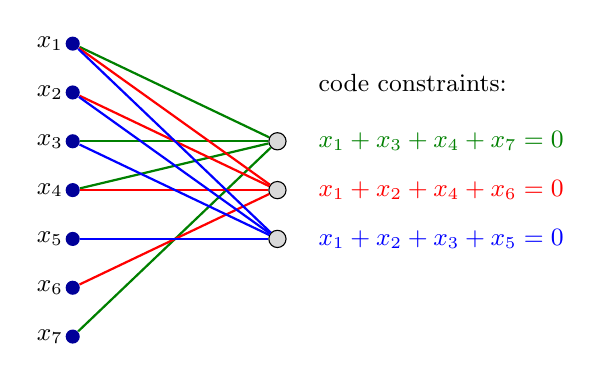
\begin{tikzpicture}[font=\small, x=1cm, y=0.62cm,
  var/.style={circle, fill=blue!60!black, inner sep=1.8pt},
  chk/.style={circle, draw=black, fill=gray!30, inner sep=2.2pt}]
% variable (input) nodes x_1..x_7
\foreach \i in {1,...,7} {
  \node[var] (x\i) at (0,-\i) {};
  \node[left] at (x\i) {$x_{\i}$};
}
% check (output) nodes, one per row of H
\node[chk] (c1) at (2.6,-3) {};
\node[chk] (c2) at (2.6,-4) {};
\node[chk] (c3) at (2.6,-5) {};
\foreach \i in {1,3,4,7} \draw[green!50!black, thick] (x\i) -- (c1);
\foreach \i in {1,2,4,6} \draw[red, thick] (x\i) -- (c2);
\foreach \i in {1,2,3,5} \draw[blue, thick] (x\i) -- (c3);
\node[anchor=west, text=green!50!black] at (3.0,-3) {$x_1+x_3+x_4+x_7=0$};
\node[anchor=west, text=red] at (3.0,-4) {$x_1+x_2+x_4+x_6=0$};
\node[anchor=west, text=blue] at (3.0,-5) {$x_1+x_2+x_3+x_5=0$};
\node[anchor=west] at (3.0,-1.8) {code constraints:};
\end{tikzpicture}
